\section{User Controlled Walking}
\label{sec::51_uc}
As the fundamental building block for the comparison to autonomous walking, we now need to investigate on user controlled walking. This enables us, in contrast to the control by a neural network, to find the best parameters for the pattern generation in a well controllable environment. These parameters will then be kept constant throughout the rest of this thesis, in order to allow for a good comparison between user controlled walking and autonomously controlled walking. Furthermore, we will rely on them to gather data for the behavioral cloning approach in section \ref{sec::523_da}.
\subsection{Benchmarking of Implementation}

\begin{figure}[h]
	\centering
	\subcaptionbox{}%
	[.4\linewidth]{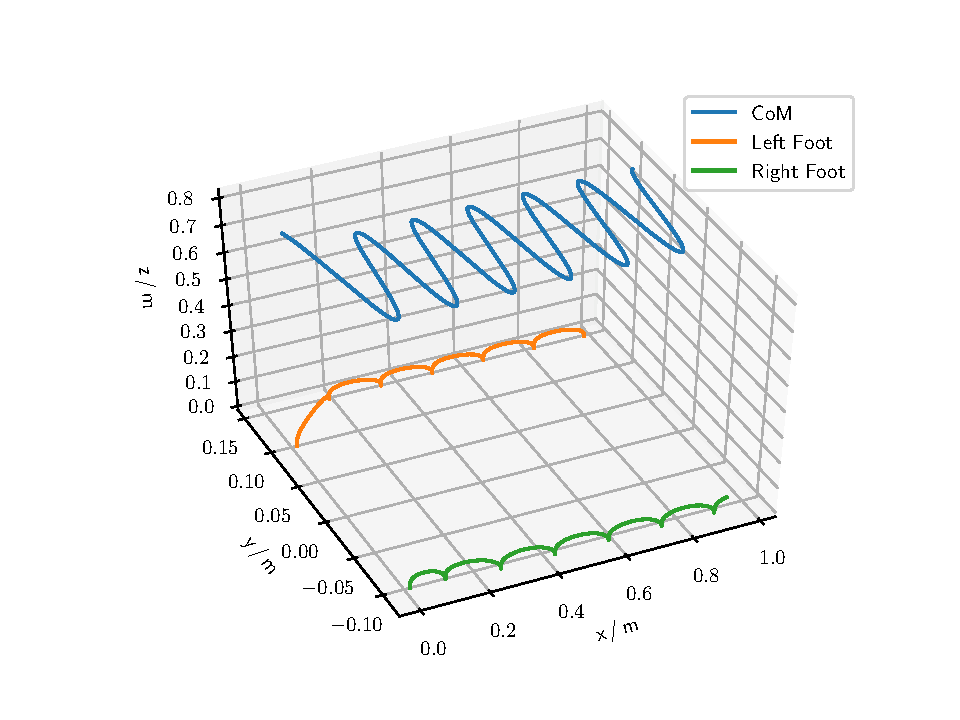
\includegraphics[scale=.35]{chapters/05_experiments/01_user_controlled_walking/01_benchmarking/nmpc_straight.pdf}}
	\subcaptionbox{}%
	[.4\linewidth]{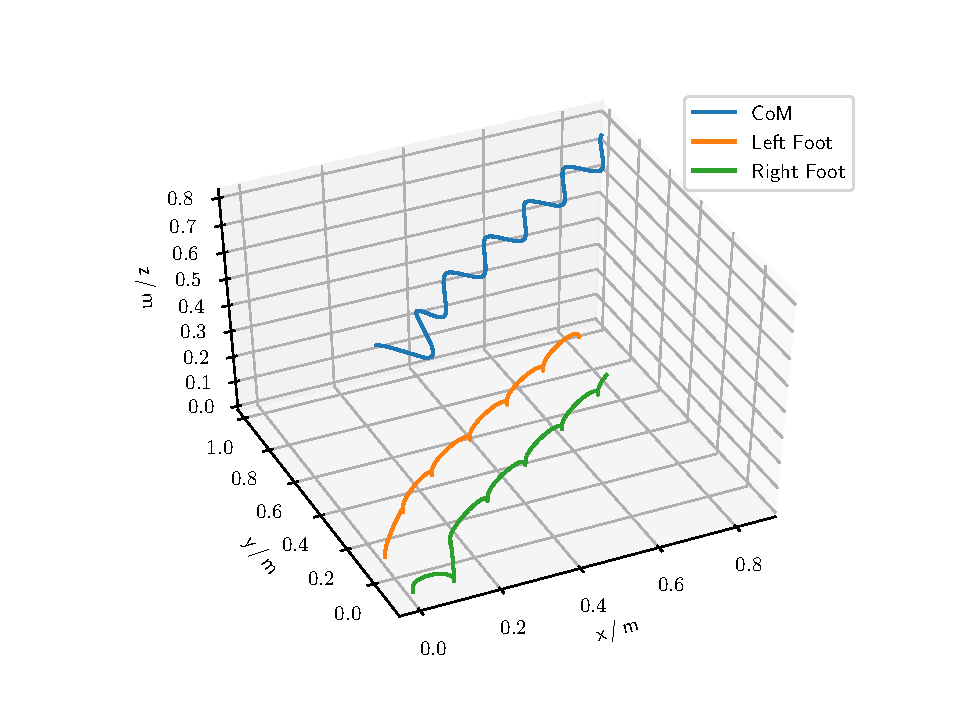
\includegraphics[scale=.35]{chapters/05_experiments/01_user_controlled_walking/01_benchmarking/nmpc_diagonal.pdf}}
	\subcaptionbox{}%
	[.4\linewidth]{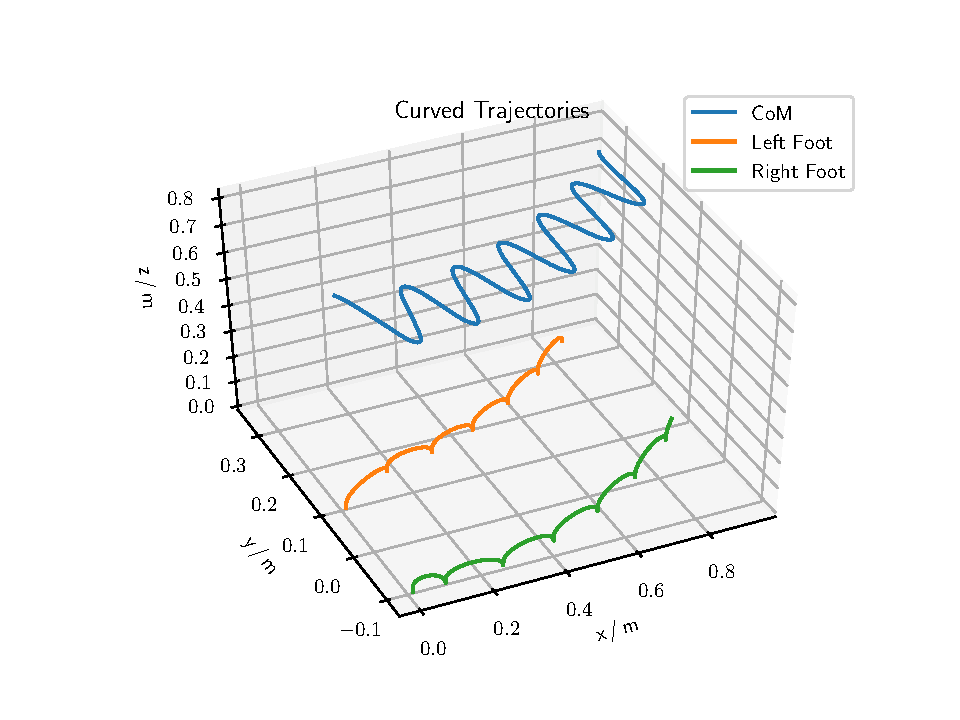
\includegraphics[scale=.35]{chapters/05_experiments/01_user_controlled_walking/01_benchmarking/nmpc_turn.pdf}}
	\subcaptionbox{}%
	[.4\linewidth]{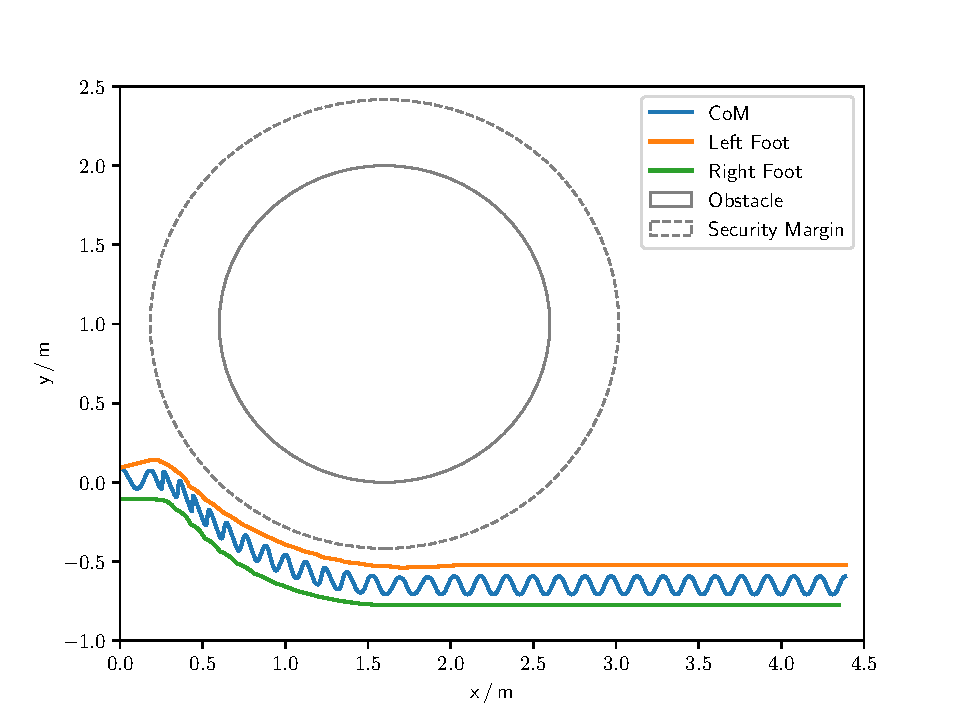
\includegraphics[scale=.35]{chapters/05_experiments/01_user_controlled_walking/01_benchmarking/nmpc_obstacle.pdf}}
	\caption{}
	\label{fig::511_benchmarking_traj}
\end{figure} 
\begin{figure}[h]
	\centering
	\subcaptionbox{Interpolated x-Trajectories}%
	[.3\linewidth]{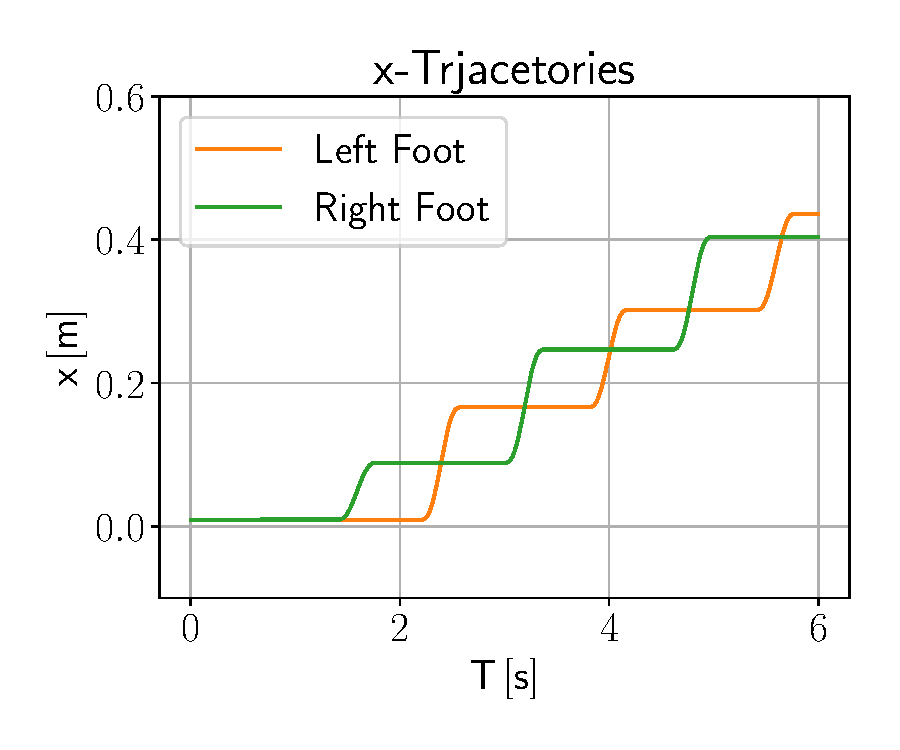
\includegraphics[scale=.3]{chapters/05_experiments/01_user_controlled_walking/01_benchmarking/interpolated_x_trajectories.pdf}}
	\subcaptionbox{Interpolated y-Trajectories}%
	[.3\linewidth]{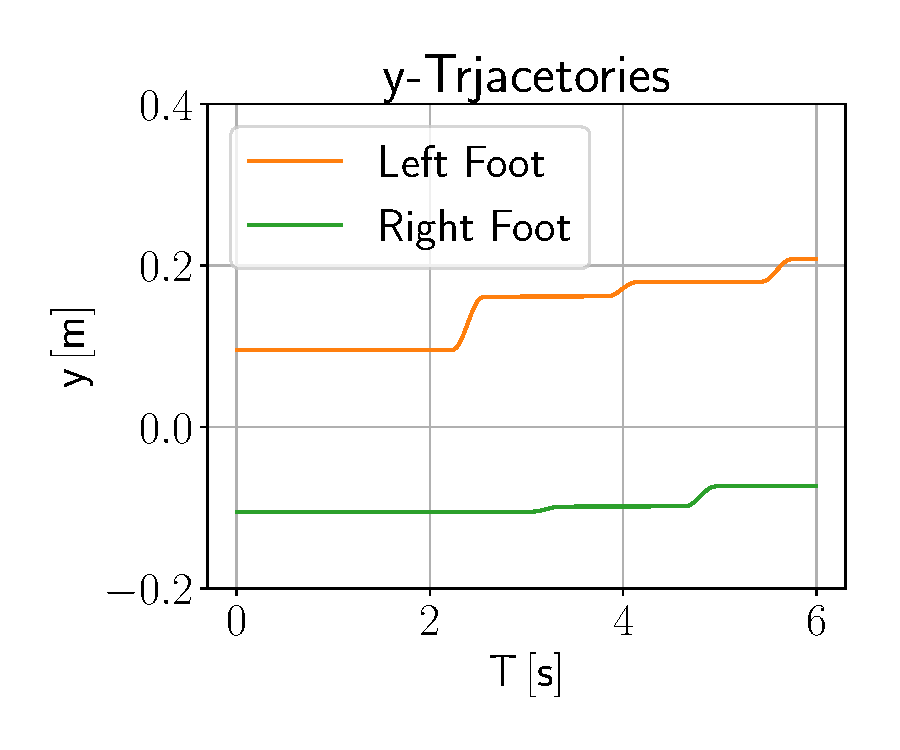
\includegraphics[scale=.3]{chapters/05_experiments/01_user_controlled_walking/01_benchmarking/interpolated_y_trajectories.pdf}}
	\subcaptionbox{Interpolated z-Trajectories}%
	[.3\linewidth]{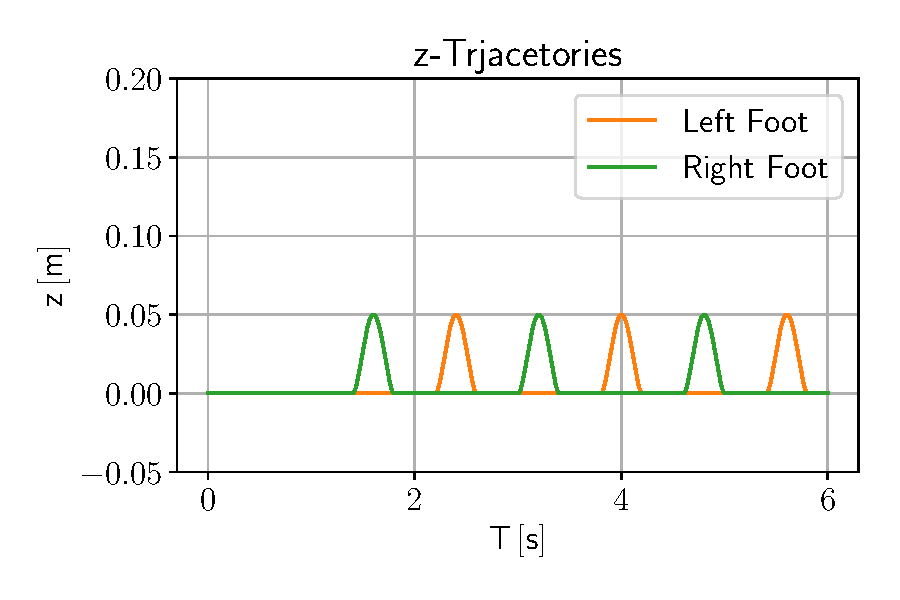
\includegraphics[scale=.3]{chapters/05_experiments/01_user_controlled_walking/01_benchmarking/interpolated_z_trajectories.pdf}}
	\caption{}
	\label{fig::511_benchmarking_inter}
\end{figure} 
\subsection{Performance in Test Environment}
\begin{figure}[h]
	\centering
	\subcaptionbox{Straight Walk - Dynamic Balance}%
	[.4\linewidth]{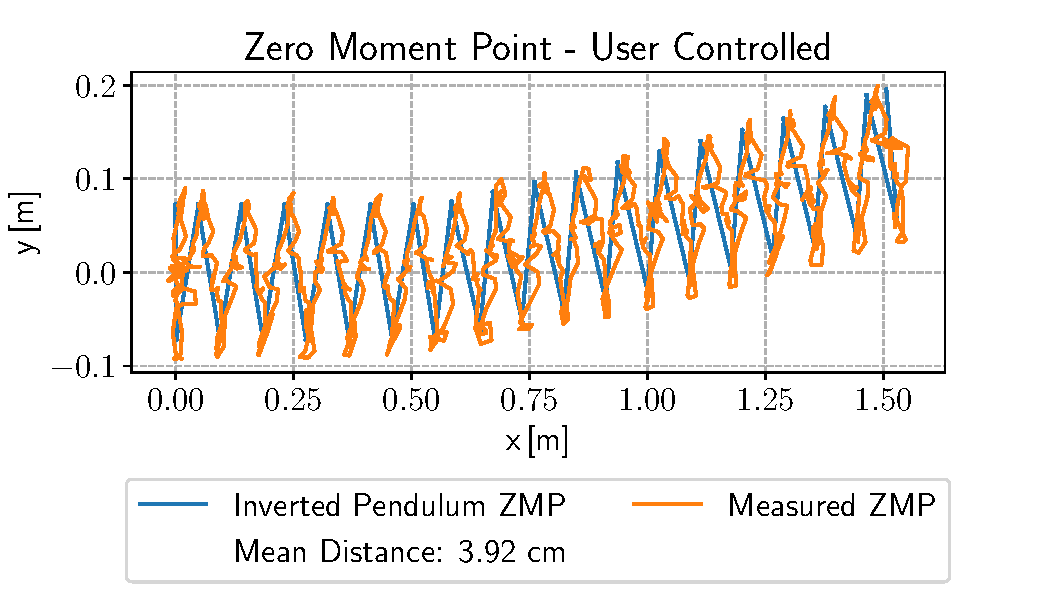
\includegraphics[scale=.35]{chapters/05_experiments/01_user_controlled_walking/02_test_environment/straight_walk_01_zmp.pdf}}
	\subcaptionbox{Straight Walk - Behavior}%
	[.4\linewidth]{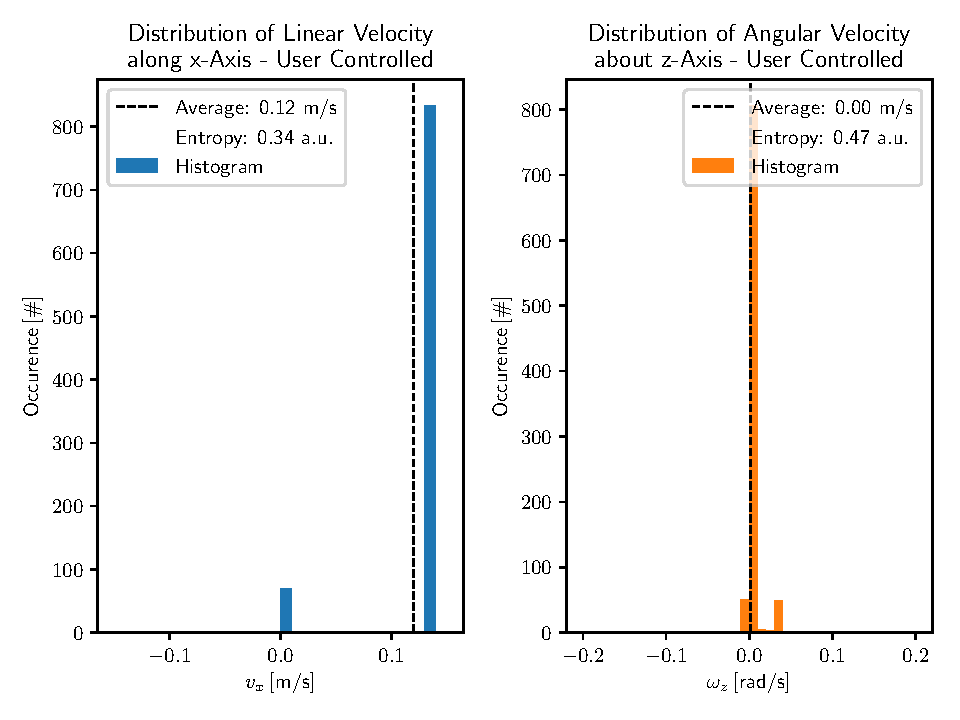
\includegraphics[scale=.35]{chapters/05_experiments/01_user_controlled_walking/02_test_environment/straight_walk_01_entropy.pdf}}
	\subcaptionbox{Curved Walk - Dynamic Balance}%
	[.4\linewidth]{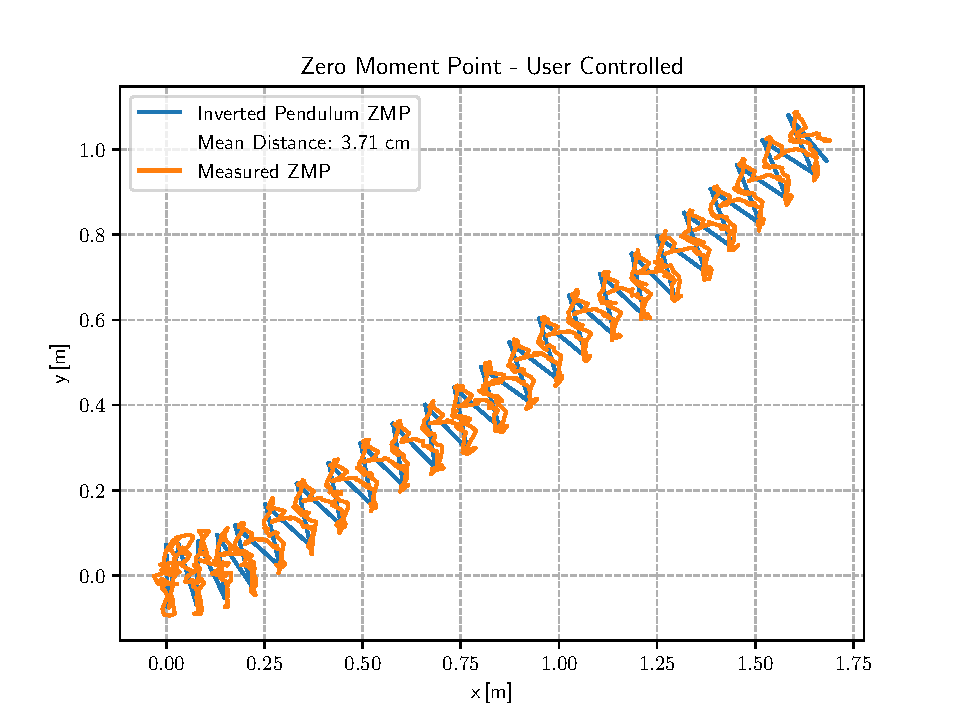
\includegraphics[scale=.35]{chapters/05_experiments/01_user_controlled_walking/02_test_environment/curved_walk_01_zmp.pdf}}
	\subcaptionbox{Curved Walk - Behavior}%
	[.4\linewidth]{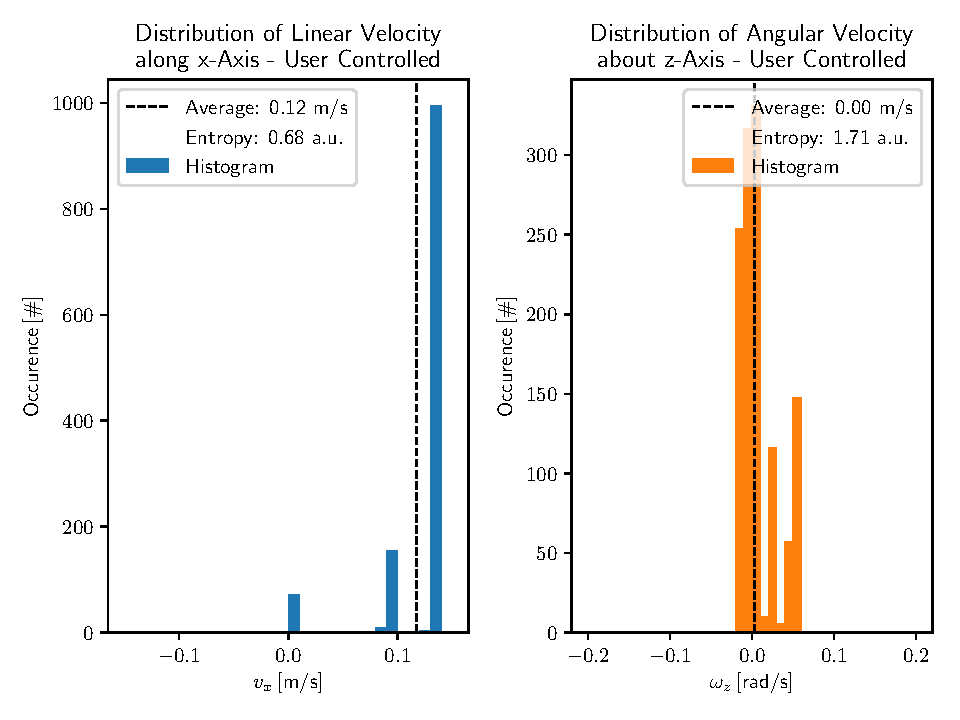
\includegraphics[scale=.35]{chapters/05_experiments/01_user_controlled_walking/02_test_environment/curved_walk_01_entropy.pdf}}
	\subcaptionbox{Obstacle Avoidance - Dynamic Balance}%
	[.4\linewidth]{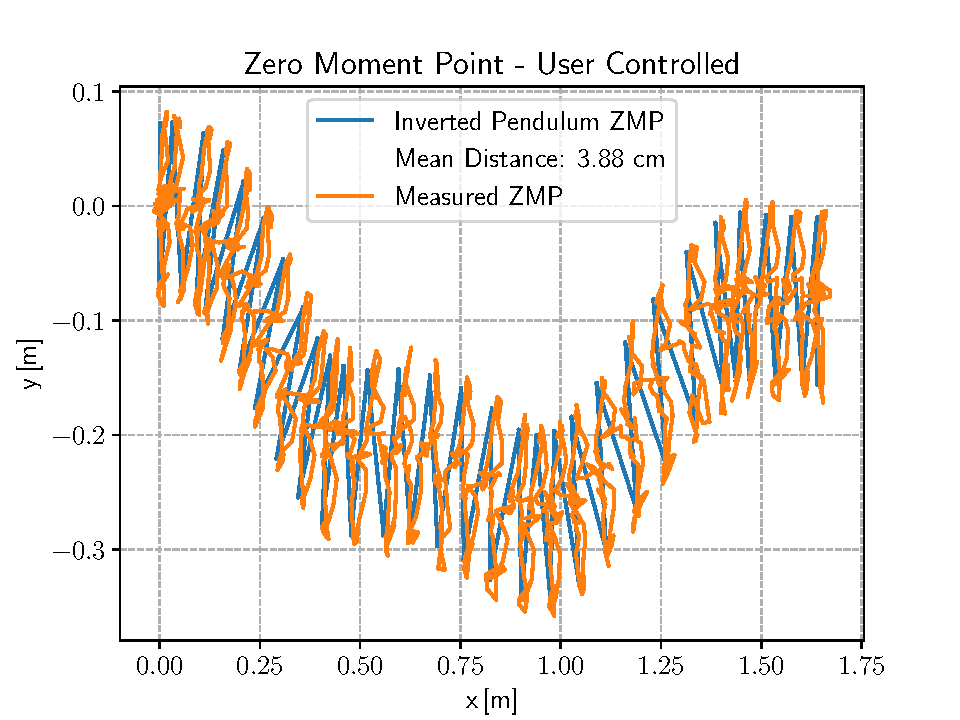
\includegraphics[scale=.35]{chapters/05_experiments/01_user_controlled_walking/02_test_environment/obstacle_walk_02_zmp.pdf}}
	\subcaptionbox{Obstacle Avoidance - Behavior}%
	[.4\linewidth]{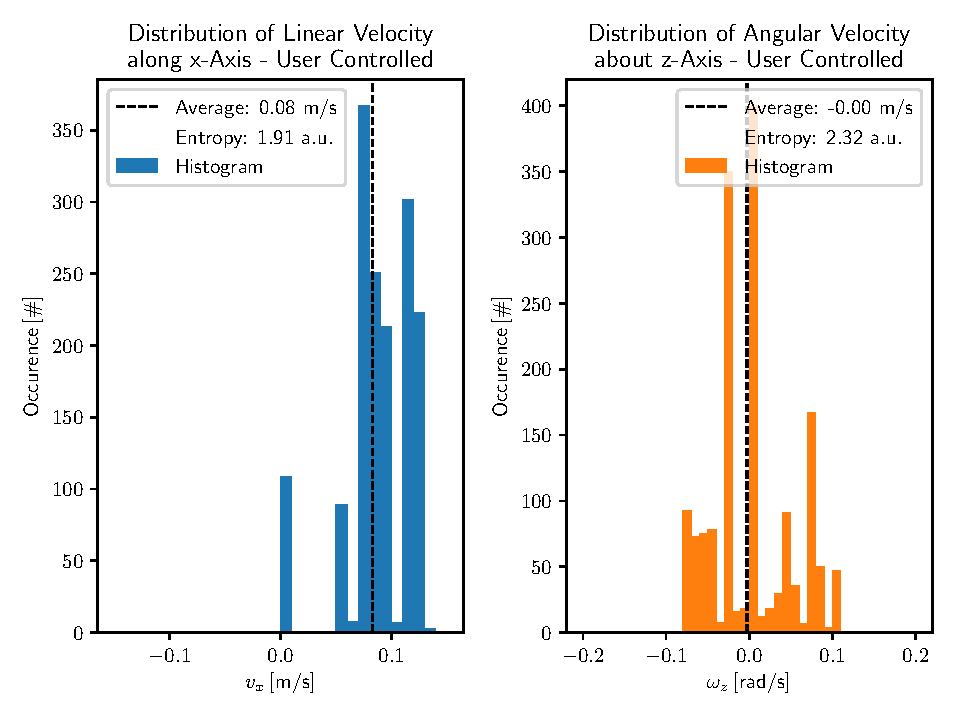
\includegraphics[scale=.35]{chapters/05_experiments/01_user_controlled_walking/02_test_environment/obstacle_walk_02_entropy.pdf}}
	\subcaptionbox{Environment Scanning - Dynamic Balance}%
	[.4\linewidth]{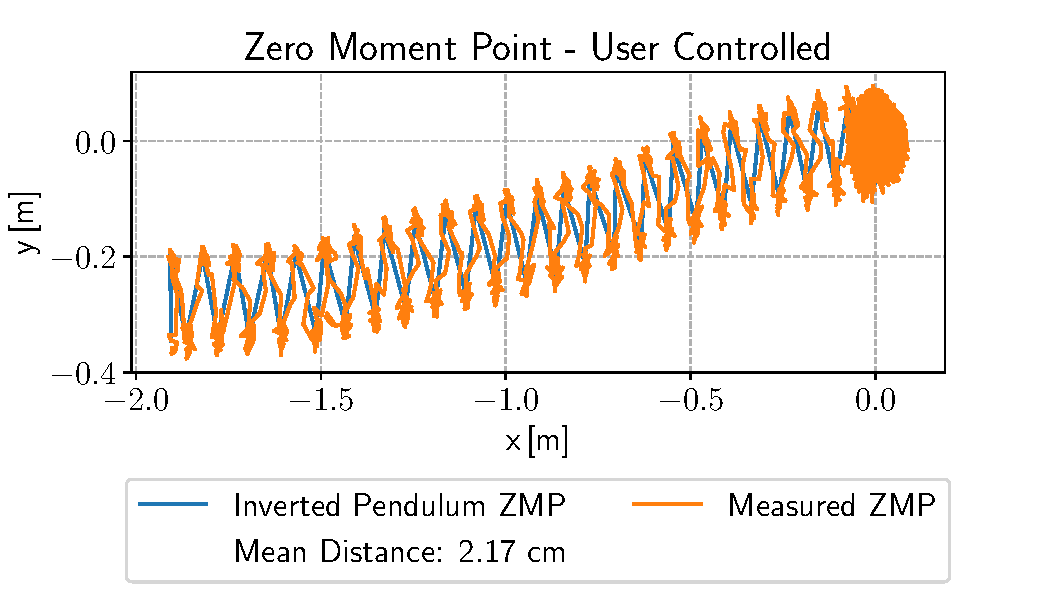
\includegraphics[scale=.35]{chapters/05_experiments/01_user_controlled_walking/02_test_environment/out_of_sight_walk_01_zmp.pdf}}
	\subcaptionbox{Environment Scanning - Behavior}%
	[.4\linewidth]{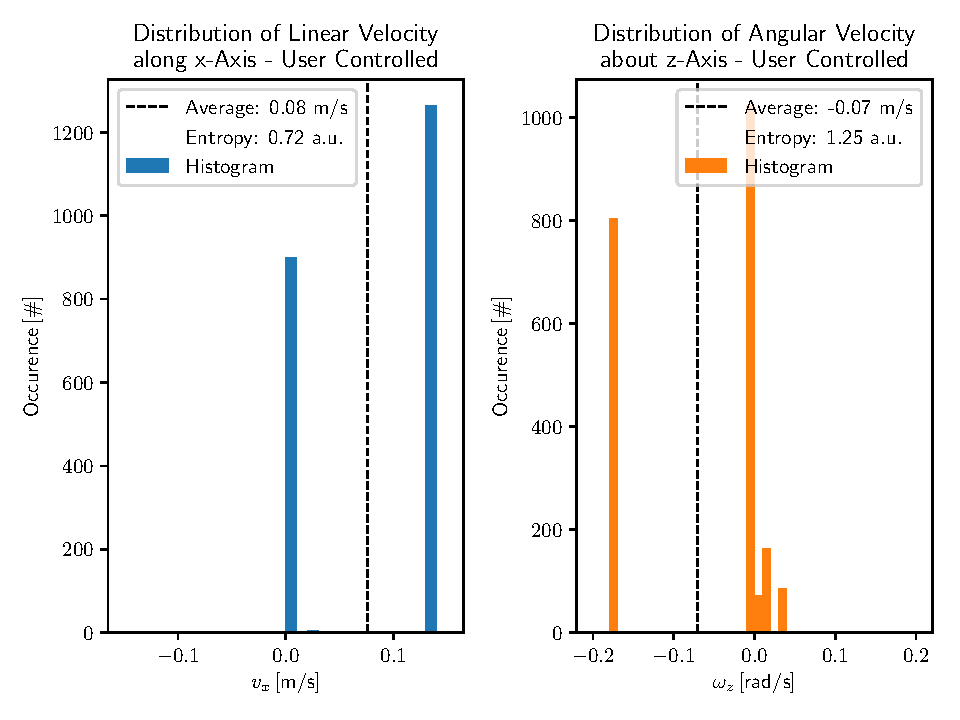
\includegraphics[scale=.35]{chapters/05_experiments/01_user_controlled_walking/02_test_environment/out_of_sight_walk_01_entropy.pdf}}
	\caption{}
	\label{fig::512_uc_basic}
\end{figure} 